\documentclass[12pt]{article}

\usepackage{graphicx}
\usepackage{paralist}
\usepackage{hyperref}
\usepackage{xspace}
\usepackage{amsfonts}
\usepackage{amsmath}
\usepackage{multirow}


\newcommand{\latex}{\LaTeX\xspace}

\oddsidemargin 0mm
\evensidemargin 0mm
\textwidth 160mm
\textheight 200mm
\renewcommand\baselinestretch{1.0}

\pagestyle {plain}
\pagenumbering{arabic}

\newcounter{stepnum}

\title{Design Specification \\ 
JobSeeker \\ 
\large Version 2}
\author{Zihao Du\\
Senni Tan\\
Gengyun Wang\\
Wenzhi Wang\\
Lab 3 Group 3\\
Computing and Software Department, Mcmaster University \\
SFWR ENG 2XB3, Software Engineering Practice and Experience:\\ Binding Theory to Practice\\
}

\begin {document}

\maketitle
\newpage

\section*{Revision Page}
\noindent By  virtue  of  submitting  this  document  we  electronically  sign  and  date  that  the  work  being  submitted  by  all  the individuals  in  the  group  is  their  exclusive  work  as  a  group  and  we  consent  to  make  available  the  application developed  through  [CS]  or  [SE]-2XB3  project,  the  reports,  presentations,  and  assignments  (not  including  my name and student number) for future teaching purposes.\\
\noindent \textbf{\emph{First revision:}}
\begin{description}
\item    Senni Tan --- Edited the title page and created the contribution table.
\item    Zihao Du --- Added the attestation and consent in Revision.
\end{description}
\noindent \textbf{\emph{Second revision:}}
\begin{description}
\item    Senni Tan --- Edited the contribution table.
\item    Zihao Du--- Edited the contribution table.
\item    Wang Wenzhi --- Edit the contribution table.
\item    Gengyun Wang --- Edited the contribution table.
\end{description}
\noindent \textbf{\emph{Third revision:}}
\begin{description}
\item    Senni Tan --- Modules MIS; Description of implementation; View of uses relationship; Internal review.
\item    Zihao Du--- Modules MIS; Description of implementation; Description of Modules; Internal review.
\item    Wang Wenzhi --- Modules MIS; Description of implementation; implementation and two UML for two most interesting classes; Internal review.
\item    Gengyun Wang --- Modules MIS; Description of implementation and trace back to requirements; Internal review.
\end{description}
\newpage

\section*{Contribution Page}

\begin{center}
\begin{tabular}{ |c|c|c|c| } 
\hline
Name & Role(s) & Contribution & Comments \\
\hline
\multirow{3}{4em}{Zihao Du} & Designer & Proposal Abstract and motivation & \\ 
& Researcher & Database of jobs & \\ 
& Designer & SRS Functional requirement  & \\ 
& ~ & Graphing algorithm implementation & \\
& ~ & Client module & \\
& Tester & Unit test for graphing algorithm & \\
& ~ & Design Specifications(refer to document revisions) & \\
\hline
\multirow{3}{4em}{Senni Tan} & Designer & Proposal I/O& \\ 
& ~ & SRS Non-functional requirement  & \\ 
& ~ & Sorting Algorithm Implementation & \\
& Tester & Unit test for sorting algorithm implementation & \\
& ~ & Design Specifications(refer to document revisions) & \\
\hline
\multirow{3}{4em}{Gengyun Wang} & Designer & Proposal Prior Work& \\ 
& ~ & SRS Assumptions, Domain  & \\ 
& ~ & Searching Algorithm Implementation & \\
& Tester & Unit test for searching algorithm implementation & \\
& ~ & Design Specifications(refer to document revisions) & \\
\hline
\multirow{3}{4em}{Wenzhi Wang} & Designer & Proposal Reference page& \\ 
& ~ & SRS  Maintenance and Development & \\ 
& ~ & Data processing implementation & \\
& Tester & Test and modify the client code implementation & \\
& ~ & Design Specifications(refer to document revisions) & \\
\hline
\end{tabular}
\end{center}

\newpage

\section*{Executive Summary}
JobSeeker is designed for potential immigrants, people new to Canada that are looking for a job and Canadian job seeker. It will provide the user positions of jobs they are interested in and show the relative information. The project is composed by five main modules; a Job module which constructs the Job ADT; a Data Process module which processes data from datasets, converts them to Job objects, stores the objects and return; a Sorting module which sorts the Job objects arrays, with the help from the Comparable module; a Searching module which does the searching on Job objects with some given conditions; and a DFS module which finds the relative jobs for a given job source in the graph constructed by the Graph ADT. The prototype of this design will be presented in the Demo module. This document gives the detail of the project design in the sections below.

\tableofcontents
\newpage

\section{Description of Modules}
The design is made up with nine modules including the client module. These modules can be divided into four categories: Data Processing, Sorting, Searching and Graphing.\\\newline Job class and Dataprocess class belongs to Data Processing, which make use of data from the database and store that into some data structures in Java. Job class defines state variables for an object Job, which is an important and fundamental object for the design. The methods in Job class are all getters. Dataprocess class takes no input and use Job class to store information from dataset into its state variable "joblist".\\\newline Sorting catagory contains two classes: Comparable and Sorting. Since we need to sort by different criteria, the Comparable class provides different compareTo methods. The Sorting class inherits these methods and use quicksort algorithm to sort the input ArrayList. \\\newline Searching catagory contains only a single module Searching.Just like Sorting class, it provides static functions instead of creating objects. It uses binary search assuming that the ArrayList is already sorted to get the kind of Job the user what and return them in an ArrayList. \\\newline The Graphing part is a trival one. It contains two classes: Graph and DFS. Graph creates an undirected graph class while DFS is an object exploring reachable nodes with depth-frist search algorithm based on a Graph class. \\\newline The client module part uses outputs of Searching, Sorting and Graphing parts. It also makes use of a class called Noc which provides a list of job catagories for user selection and demostration.
\begin{center}
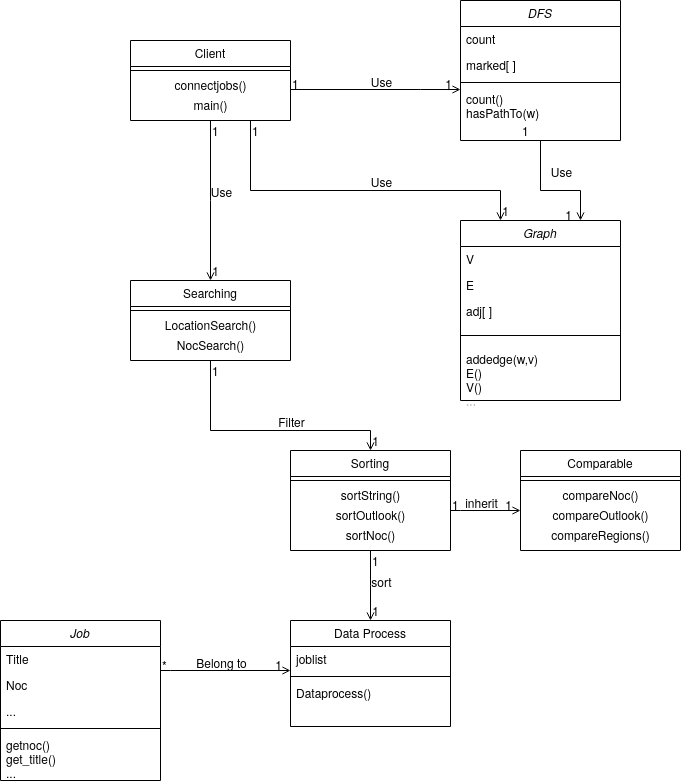
\includegraphics[width=0.8\textwidth]{UML Diagram.png}
\end{center}
\newpage
\section{Detailed description of interfaces}
%% Job
\section* {Job ADT Module}

\subsection*{Template Module}

Job

\subsection* {Uses}

N/A

\subsection* {Syntax}

\subsubsection* {Exported Types}

Job = ?

\subsubsection* {Exported Access Programs}

\begin{tabular}{| l | l | l | l |}
\hline
\textbf{Routine name} & \textbf{In} & \textbf{Out} & \textbf{Exceptions}\\
\hline
Job & seq of $\mathbb{Z}$, String,$\mathbb{Z}$,$\mathbb{Z}$,String,$\mathbb{Z}$,String  & Job & \\
\hline
get\_noc & $\mathbb{Z}$ & $\mathbb{Z}$ &\\
\hline
getnoc & ~ & seq of $\mathbb{Z}$ &\\
\hline
get\_title & ~ & String &\\
\hline
get\_location & ~ & String &\\
\hline
get\_region & ~ & $\mathbb{Z}$ &\\
\hline
get\_outlook & ~ & $\mathbb{Z}$ &\\
\hline
get\_year & ~ & $\mathbb{Z}$ &\\
\hline
get\_regions & ~ & String &\\
\hline
getInfo & ~ & String &\\
\hline
getbriefInfo & ~ & String &\\
\hline
printInfo & ~ &~ &\\
\hline
printbriefInfo & ~ &~ &\\
\hline
\end{tabular}

\subsection* {Semantics}

\subsubsection* {State Variables}

$noc$: seq of $\mathbb{Z}$\\
$title$: String\\
$outlook$: $\mathbb{Z}$\\
$year$: $\mathbb{Z}$\\
$region$: $\mathbb{Z}$\\
$regions$: String\\
$location$: String\\

\subsubsection* {State Invariant}

None

\subsubsection* {Assumptions}

The constructor Job is called for each object instance before any other
access routine is called for that object.  The constructor cannot be called on
an existing object.

\subsubsection* {Access Routine Semantics}

Job($noc, title, outlook, year, location, region, regions$):
\begin{itemize}
\item transition: $noc, title, outlook, year, location, region, regions := noc, title, outlook, year, location, region, regions$
\item output: $out := \mathit{self}$
\item exception: None
\end{itemize}

\noindent get\_noc($index$):
\begin{itemize}
\item output: $out := noc[index]$
\item exception: None
\end{itemize}

\noindent getnoc( ):
\begin{itemize}
\item output: $out := noc[0]*1000+noc[1]*100+noc[2]*10+noc[3]$
\item exception: None
\end{itemize}

\noindent get\_title( ):
\begin{itemize}
\item output: $out := title$
\item exception: None
\end{itemize}

\noindent get\_location( ):
\begin{itemize}
\item output: $out := location$
\item exception: None
\end{itemize}

\noindent get\_region( ):
\begin{itemize}
\item output: $out := region$
\item exception: None
\end{itemize}

\noindent get\_outlook( ):
\begin{itemize}
\item output: $out := outlook$
\item exception: None
\end{itemize}

\noindent get\_year( ):
\begin{itemize}
\item output: $out := year$
\item exception: None
\end{itemize}

\noindent get\_regions( ):
\begin{itemize}
\item output: $out := regions$
\item exception: None
\end{itemize}

\noindent printbriefInfo( ):
\begin{itemize}
\item exception: None
\end{itemize}

\noindent getbriefInfo( ):
\begin{itemize}
\item output: $out := "Job\ title: "+this.get\_title()+"    Noc\ \_ "+this.get\_noc(0)+" "+ this.get\_noc(1)+" "+this.get\_noc(2)+" "+this.get\_noc(3)$
\item exception: None
\end{itemize}

\noindent printInfo( ):
\begin{itemize}
\item exception: None
\end{itemize}

\noindent getInfo( ):
\begin{itemize}
\item output: $out := "Job\ title: "+this.get\_title()+"\backslash nNoc \_ "+this.get\_noc(0)+" "+ this.get\_noc(1)+" "+this.get\_noc(2)+" "+this.get\_noc(3)+"\backslash nOutlook: "+this.get\_outlook()+"\backslash nProvince: "+this.get\_location()+"\backslash nEcon region code: "+this.get\_region()+"\backslash nEcon\ region\ name: "+this.get\_regions()+"\backslash nYear "+this.get\_year()+"\backslash n"$
\item exception: None
\end{itemize}
%%End Job
\newpage
%%data process
\section* {DataProcess Module}

\subsection*{Module}

DataProcess

\subsection* {Uses}

Job

\subsection* {Syntax}

\subsubsection* {Exported Types}

DataProcess = ?

\subsubsection* {Exported Access Programs}

\begin{tabular}{| l | l | l | l |}
\hline
\textbf{Routine name} & \textbf{In} & \textbf{Out} & \textbf{Exceptions}\\
\hline
DataProcess &~ & ~ &FileNotFoundException \\
\hline
get\_data &~ & seq of Job & \\
\hline

\end{tabular}

\subsection* {Semantics}

\subsubsection* {State Variables}

$dataset$: seq of Job\\


\subsubsection* {State Invariant}

None

\subsubsection* {Assumptions}

The constructor DataProcess is called only once for only one object for reading the dataset files.

\subsubsection* {Access Routine Semantics}

DataProcess( ):
\begin{itemize}
\item transition: $dataset + Job$
\item output: $out := \mathit{self}$
\item exception: FileNotFoundException
\end{itemize}

get\_data( ):
\begin{itemize}
\item output: $out := dataset$
\item exception: None
\end{itemize}

%%end data process

\newpage
\section* {Comparator Module}

\subsection* {Module}

Comparable

\subsection* {Uses}

Job

\subsection* {Syntax}

\subsubsection* {Exported Access Programs}

\begin{tabular}{| l | l | l | p{6cm} |}
\hline
\textbf{Routine name} & \textbf{In} & \textbf{Out} & \textbf{Exceptions}\\
\hline
CompareString & Job, Job & $\mathbb{Z}$ & \\
\hline
CompareOutlook & Job, Job & $\mathbb{Z}$ & \\
\hline
CompareNOC & Job, Job & $\mathbb{Z}$ & \\
\hline
CompareRegionS & Job, Job & $\mathbb{Z}$ & \\
\hline
\end{tabular}

\subsection* {Semantics}

\subsubsection* {Access Routine Semantics}

\noindent CompareString(a, b):
\begin{itemize}
\item output: $out := $ a.get\_title.compareTo(b.get\_title)
\item exception: None
\end{itemize}
\noindent \textit{// compareTo is a build in method to compare String in lexgraphical order.}\\

\noindent CompareOutlook(a, b):
\begin{itemize}
\item output: $out :=$ (a.get\_outlook $>$ b.get\_outlook) $\Rightarrow$ 1 $|$ (a.get\_outlook $<$ b.get\_outlook) $\Rightarrow$ -1 $|$ 0
\item exception: None
\end{itemize}

\noindent CompareNOC(a, b):
\begin{itemize}
\item output: $out :=$ (a.get\_noc(0) $>$ b.get\_noc(0)) $\Rightarrow$ 1 $|$ (a.get\_noc(0) $<$ b.get\_noc(0)) $\Rightarrow$ -1 $|$ 0
\item exception: None
\end{itemize}

\noindent CompareRegionS(a, b):
\begin{itemize}
\item output: $out := $ a.get\_regions.compareTo(b.get\_regions)
\item exception: None
\end{itemize}
\noindent \textit{// compareTo is a build in method to compare String in lexgraphical order.}\\

\newpage

\section* {Sorting Module}

\subsection* {Module}

Sorting

\subsection* {Uses}

Comparable

\subsection* {Syntax}

\subsubsection* {Exported Access Programs}

\begin{tabular}{| l | l | l | p{6cm} |}
\hline
\textbf{Routine name} & \textbf{In} & \textbf{Out} & \textbf{Exceptions}\\
\hline
sortString & Seq of Job & ~ & \\
\hline
sortOutlook & Seq of Job & ~ & \\
\hline
sortNOC & Seq of Job & ~ & \\
\hline
sortRegionS & Seq of Job & ~ & \\
\hline
\end{tabular}

\subsection* {Semantics}

\subsubsection* {Access Routine Semantics}

\noindent sortString(a):
\begin{itemize}
\item transition: sortString(a, 0, $|a|$-1)
\item exception: None
\end{itemize}

\noindent sortOutlook(a):
\begin{itemize}
\item transition: sortOutlook(a, 0, $|a|$-1)
\item exception: None
\end{itemize}

\noindent sortNOC(a):
\begin{itemize}
\item transition: sortNOC(a, 0, $|a|$-1)
\item exception: None
\end{itemize}

\noindent sortRegionS(a):
\begin{itemize}
\item transition: sortRegionS(a, 0, $|a|$-1)
\item exception: None
\end{itemize}

\newpage

\section* {Searching Module}
\subsection*{Module}

Searching

\subsection* {Uses}

Job

\subsection* {Syntax}
\subsubsection* {Exported Constants}

None
\subsubsection* {Exported Types}

Searching = seq of Job

\subsubsection* {Exported Access Programs}

\begin{tabular}{| l | l | l | l |}
\hline
\textbf{Routine name} & \textbf{In} & \textbf{Out} & \textbf{Exceptions}\\
\hline
LocationSearch & seq of Job, String & seq of Job & \\
\hline
NocSearch & seq of Job, $\mathbb{Z}$ & seq of Job & \\
\hline
\end{tabular}

\subsection* {Semantics}

\subsubsection* {State Variables}

None

\subsubsection* {State Invariant}

None
\subsubsection* {Assumptions}

None

\subsubsection* {Access Routine Semantics}

\noindent LocationSearch($jobs$, $location$):
\begin{itemize}
\item output: $out := \langle e: Job | e \in jobs \wedge e.get\_regions() = location : e \rangle $ \textit{Return a sequence of all the elements from input location in the input sequence jobs}
\item exception: None
\end{itemize}
\noindent \textit{// get\_regions() is a method from Job ADT class.}\\

\noindent NocSearch($jobs$, $noc$):
\begin{itemize}
\item output: $out := \langle e: Job | e \in jobs \wedge e.get\_noc(0) = noc : e \rangle $ \textit{Return a sequence of all the elements with same input noc number in the input sequence jobs}
\item exception: None
\end{itemize}
\noindent \textit{// get\_noc(int index) is a method from Job ADT class.}\\

\newpage


\section* {Graph Module}

\subsection*{Module}

Graph

\subsection* {Uses}

N/A

\subsection* {Syntax}

\subsubsection* {Exported Constants}

None

\subsubsection* {Exported Types}

Graph = ?

\noindent \textit{//An undirected graph with unweighed edges}

\subsubsection* {Exported Access Programs}

\begin{tabular}{| l | l | l | l |}
\hline
\textbf{Routine name} & \textbf{In} & \textbf{Out} & \textbf{Exceptions}\\
\hline
Graph & $\mathbb{Z}$ & Graph & NegativeArraySizeException\\
\hline
addedge & $\mathbb{N}$, $\mathbb{N}$ & ~ & IllegalArgumentException\\
\hline
V & ~ & $\mathbb{N}$ & ~\\
\hline
E & ~ & $\mathbb{N}$ & ~\\
\hline
adj & $\mathbb{N}$ & Seq of $\mathbb{N}$ & IllegalArgumentException\\
\hline
\end{tabular}


\subsection* {Semantics}

\subsubsection* {State Variables}

$V$: $\mathbb{N}$\\
$E$: $\mathbb{N}$\\
$adj$: Seq of Seq of $\mathbb{N}$

\subsubsection* {State Invariant}

None
\subsubsection* {Assumptions}

The constructor Graph is called for each object instance before any other access routine is called for that object.  The constructor cannot be called on
an existing object.

\subsubsection* {Access Routine Semantics}

\noindent \textit{//Constructor of Graph class}\\
Graph($v$):
\begin{itemize}
\item transition: $V, E, adj := v, 0, \mbox{Seq of Seq of   }\mathbb{N}\mbox{ with length v}$
\item output: $out := \mathit{self}$
\item exception: $exc := v < 0 \Rightarrow \mbox{NegativeArraySizeException}$
\end{itemize}

\noindent \textit{//Connect vertex w and vertex v}\\
\noindent addedge($w$, $v$):
\begin{itemize}
\item transition: $E, adj[w], adj[v] := E + 1, adj[w] \,||\, v, adj[v] \,||\, w$
\item exception: $exc := w < 0 \lor w > V  \lor v < 0 \lor v \lor V \Rightarrow \mbox{IllegalArgumentException}$
\end{itemize}

\noindent \textit{//Getter, get the number of edges}\\
\noindent E():
\begin{itemize}
\item output: $out := E$
\item exception: None
\end{itemize}

\noindent \textit{//Getter, get the number of vertices}\\
\noindent V():
\begin{itemize}
\item output: $out := V$
\item exception: None
\end{itemize}

\noindent \textit{//Getter, get a list of nodes that are conneted with vertex v}\\
\noindent adj($v$):
\begin{itemize}
\item output: $out := adj[v]$
\item exception: $exc := v < 0 \lor v > V \Rightarrow \mbox{IllegalArgumentException}$
\end{itemize}
\newpage

\section* {DFS Module}

\subsection*{Module}

DFS

\subsection* {Uses}

Graph

\subsection* {Syntax}

\subsubsection* {Exported Constants}

None

\subsubsection* {Exported Types}

DFS = ?

\noindent \textit{//Detect the reachable vertices from a source vertex}

\subsubsection* {Exported Access Programs}

\begin{tabular}{| l | l | l | l |}
\hline
\textbf{Routine name} & \textbf{In} & \textbf{Out} & \textbf{Exceptions}\\
\hline
DFS & Graph, $\mathbb{N}$  & DFS & IllegalArgumentException\\
\hline
hasPathTo & $\mathbb{N}$ & $\mathbb{B}$ & IllegalArgumentException\\
\hline
count & ~ & $\mathbb{N}$ & ~\\
\hline
\end{tabular}


\subsection* {Semantics}

\subsubsection* {State Variables}

$count$: $mathbb{N}$\\
$marked$: Seq of $\mathbb{B}$

\subsubsection* {State Invariant}

None
\subsubsection* {Assumptions}

The constructor DFS is called for each object instance before any other access routine is called for that object.  The constructor cannot be called on
an existing object.

\subsubsection* {Access Routine Semantics}

\noindent \textit{//Constructor of DFS class}\\
Graph($g$, $s$):
\begin{itemize}
\item transition: $count, \mbox{marked} := \mbox{number of reachable nodes}, \mbox{Seq of }\mathbb{B}\mbox{ recording if a vertex is reachable}$
\item output: $out := \mathit{self}$
\item exception: $exc := s < 0 \lor s >= g.V() \Rightarrow \mbox{IllegalArgumentException}$
\end{itemize}

\noindent \textit{//Determine if vertex w is reachable from the source vertex}\\
\noindent hasPathTo($w$):
\begin{itemize}
\item output: $out := marked[w]$
\item exception: $exc := w < 0 \lor w >= V \Rightarrow \mbox{IllegalArgumentException}$
\end{itemize}

\noindent \textit{//Getter, get the number of reachable vertices}\\
\noindent count():
\begin{itemize}
\item output: $out := count$
\item exception: None
\end{itemize}
\newpage

\section{View of uses relationship}
\subsection*{Uses Hierarchy}
\begin{center}
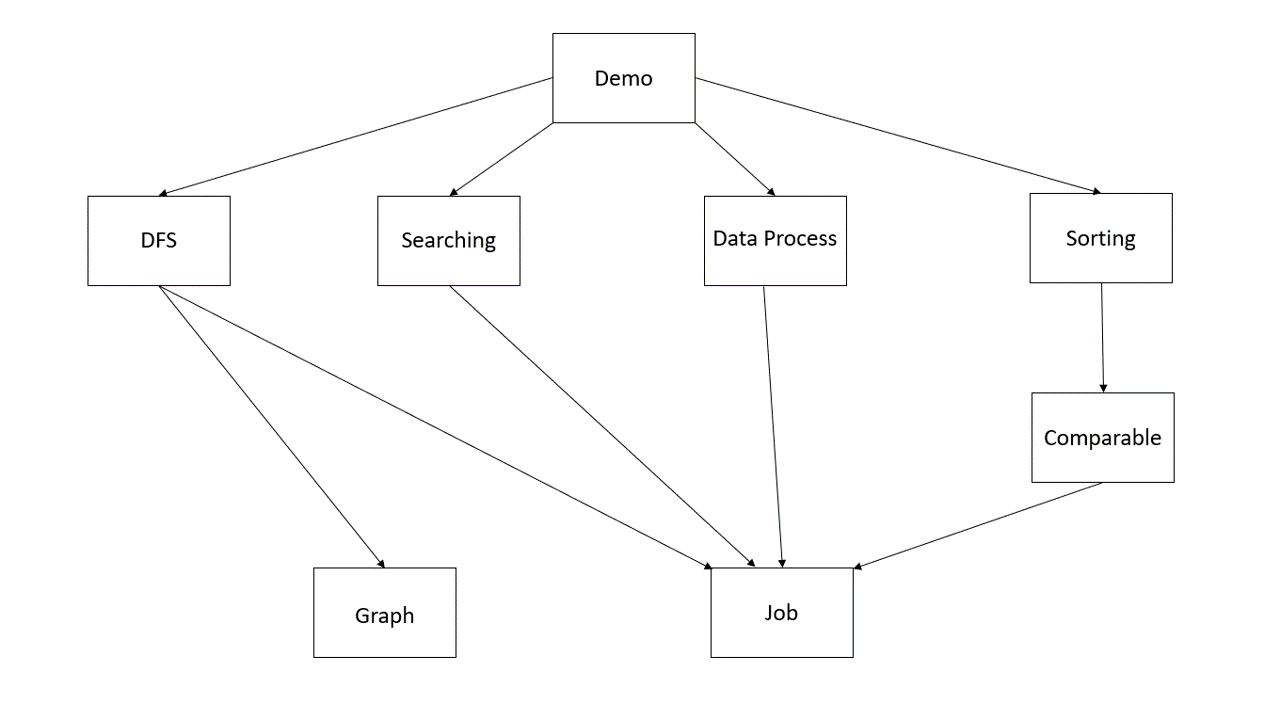
\includegraphics[scale = 0.5]{usesHierarchy.png}
\end{center}
\subsection*{Use case}
\begin{center}
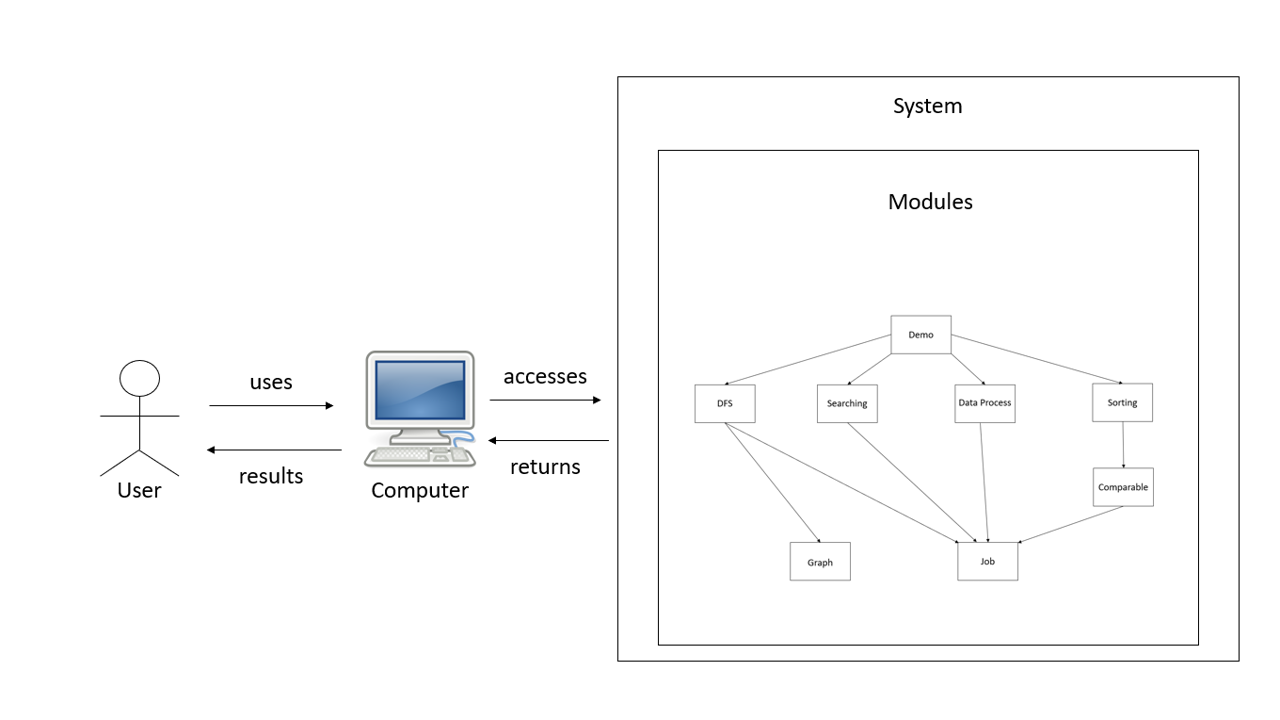
\includegraphics[scale = 0.5]{useCase.png}
\end{center}
\section{Trace back to requirements}

Demo Module (User Interface) :  This module is used to do data processing operation which uses methods from DataProcess Module to read data from database files, and store data as expected type (Job ADT). Then it will give users instructions to use methods from other modules to sort, search, and create graph for the expected data. Demo Module satisfies the I/O requirements and User Interface requirements addressed in functional requirements. If users give unavailable inputs during using, the wrong inputs will not be taken and error messages will be displayed. So it also supports the robustness, usability, and understandability addressed in non-functional requirements.\\\newline 
DataProcess Module: As mentioned above, this module is used to read data from database files, and store data as expected type (Job ADT). It satisfies the I/O requirements addressed in functional requirements. \\\newline
Job ADT Module: This module is used to build the ADT from the data in database files. The Job ADT is important to correctly use methods from other Modules like Sort, Searching, and Graph. 
Because the programmer provided detailed comments, thus the code is easy to understand and modify. So Job Module supports the understandability and maintainability addressed in non-functional requirements.\\\newline
Comparator Module: This module is used to compare the comparable attributes (like job name, noc-code) of Job ADT. Sort module will use methods from this module to sort the dataset based on the selected attribute. The code includes clear doxygen comments. Therefore it is easy to understand and modify. Comparator Module supports the understandability and maintainability addressed in non-functional requirements.\\\newline
Sort Module: This module is used to sort the dataset based on String, Outlook, NOC, and Regions by quick sort. Therefore it satisfies the sorting requirements addressed in functional requirements. Because it uses quick sort algorithm, so the performance requirements addressed in nonfunctional requirements is supported. The programmers also did Junit tests for this module, the correctness of results can be promised. Also, this programmer provided detailed comments in code for others to read and understand the code. Therefore the understandability and accuracy addressed in non-functional requirements are also satisfied.\\\newline
Searching Module: This module is used to search the expected Job set based on the given location or given noc number by using binary search. Binary search algorithm can support the performance requirements. And like sort module, the code of this module has clear comments and Junit tests to ensure the understandability and accuracy.\\\newline
Graph Module: This module is an ADT class used to create an undirected graph. Because the programmer provided detailed comments, thus the code is easy to understand and modify. So Job Module supports the understandability and maintainability addressed in non-functional requirements.\\\newline
DFS Module: This module is used detect the reachable vertices from a source graph and source vertex by depth-first search. The algorithm satisfies the the performance requirements. Like above modules, the code of this module has clear comments and Junit tests to ensure the understandability and accuracy.\\\newline
Overall: The product satisfies all the functional requirements. By the description above, the product also supports the reliability, robustness, performance, usability, maintainability, understandability, and accuracy. Besides, all the codes are implemented by Java, therefore the product can run on OS such as Windows, Mac OS, and Linux. Thus the portability is also supported.

\section{Description of implementation}
\section* {DFS Module}

\subsection*{Module}

DFS

\subsection* {Uses}

Graph

\subsection*{Local Functions}

\noindent dfs: $Graph \times \mathbb{N}$\\
\noindent \textit{//The private dfs method recursively call itself to detect deeper layer of the graph until it hits a sink vertex, then it will turn back to the previous layer and detect again. It updates the state variable "count" and "marked[]" to avoid repeatation of exploration}\\

\newpage

\section* {Sorting Module}

\subsection* {Module}

Sorting

\subsection* {Uses}

Comparable

\subsection*{Local Functions}

\noindent exch: Seq of Job $\times$ $\mathbb{Z} \times \mathbb{Z}$  $ \rightarrow $ None\\
\noindent $\mbox{exch}(a, i, j) \equiv$ exchange a[i] and a[j] in the array\\

\noindent sortString: Seq of Job $\times$ $\mathbb{Z} \times \mathbb{Z}$ $ \rightarrow $ None\\
\noindent $\mbox{sortString}(a, lo, hi) \equiv$ (hi $<=$ lo) $\Rightarrow$ return $|$ sortString(a, lo, j-1) \&\& sortString(a, j+1, hi) where j = partitionString(a, lo, hi)\\

\noindent partitionString: Seq of Job $\times$ $\mathbb{Z} \times \mathbb{Z}$ $ \rightarrow $ None\\
\noindent $\mbox{partitionString}(a, lo, hi) \equiv$ partition on array $a$ using ComapreString, see detail in code\\

\noindent sortOutlook: Seq of Job $\times$ $\mathbb{Z} \times \mathbb{Z}$ $ \rightarrow $ None\\
\noindent $\mbox{sortOutlook}(a, lo, hi) \equiv$ (hi $<=$ lo) $\Rightarrow$ return $|$ sortOutlook(a, lo, j-1) \&\& sortOutlook(a, j+1, hi) where j = partitionOutlook(a, lo, hi)\\

\noindent partitionOutlook: Seq of Job $\times$ $\mathbb{Z} \times \mathbb{Z}$ $ \rightarrow $ None\\
\noindent $\mbox{partitionOutlook}(a, lo, hi) \equiv$ partition on array $a$ using ComapreOutlook, see detail in code\\

\noindent sortNOC: Seq of Job $\times$ $\mathbb{Z} \times \mathbb{Z}$ $ \rightarrow $ None\\
\noindent $\mbox{sortNOC}(a, lo, hi) \equiv$ (hi $<=$ lo) $\Rightarrow$ return $|$ sortNOC(a, lo, j-1) \&\& sortNOC(a, j+1, hi) where j = partitionNOC(a, lo, hi)\\

\noindent partitionNOC: Seq of Job $\times$ $\mathbb{Z} \times \mathbb{Z}$ $ \rightarrow $ None\\
\noindent $\mbox{partitionNOC}(a, lo, hi) \equiv$ partition on array $a$ using ComapreNOC, see detail in code\\

\noindent sortRegionS: Seq of Job $\times$ $\mathbb{Z} \times \mathbb{Z}$ $ \rightarrow $ None\\
\noindent $\mbox{sortRegionS}(a, lo, hi) \equiv$ (hi $<=$ lo) $\Rightarrow$ return $|$ sortRegionS(a, lo, j-1) \&\& sortRegionS(a, j+1, hi) where j = partitionRegionS(a, lo, hi)\\

\noindent partitionRegionS: Seq of Job $\times$ $\mathbb{Z} \times \mathbb{Z}$ $ \rightarrow $ None\\
\noindent $\mbox{partitionRegionS}(a, lo, hi) \equiv$ partition on array $a$ using ComapreRegionS, see detail in code\\

\section* {Searching Module}
\subsection*{Module}

Searching

\subsection* {Uses}

Job

\subsection*{Local Functions}

\noindent Location\_Search: Seq of Job $\times$ String  $ \rightarrow $ $\mathbb{N}$\\
\noindent $\text{Location\_Search}(jobs, location) \equiv (m: \mathbb{N} | m \in [0 .. |jobs|-1 \wedge jobs.get(m).get\_regions() = location]
: m)$\\

\noindent \textit{//The private Location\_Search method is based on binary searching algorithm. It will first create two int variables, $l = 0$ and $r = jobs.size()-1$. Then it will process a while loop : create a int variable $m = l + (r - l) \div 2$, then it will create another int variable $res = noc.compareTo(jobs.get(m).get\_noc(0))$. If $res = 0$, return m; if $res < 0$, then $r = m-1$, continue the loop; if $res > 0$, then $l = m + 1$, continue the loop.}\\

\noindent noc\_Search: Seq of Job $\times$ $\mathbb{Z}$  $ \rightarrow $ $\mathbb{N}$\\
\noindent $\text{noc\_Search}(jobs, noc) \equiv (m: \mathbb{N} | m \in [0 .. |jobs|-1] \wedge jobs.get(m).get\_noc(0) = noc
: m)$\\

\noindent \textit{//The private Location\_Search method is based on binary searching algorithm. It will first create two int variables, $l = 0$ and $r = jobs.size()-1$. Then it will process a while loop : create a int variable $m = l + (r - l) \div 2$, then it will create another int variable $res = location.compareTo(jobs.get(m).get\_regions())$. If $res = 0$, return m; if $res < 0$, then $r = m-1$, continue the loop; if $res > 0$, then $l = m + 1$, continue the loop.}\\
\begin{center}
\noindent state machine diagram of DataProcess class
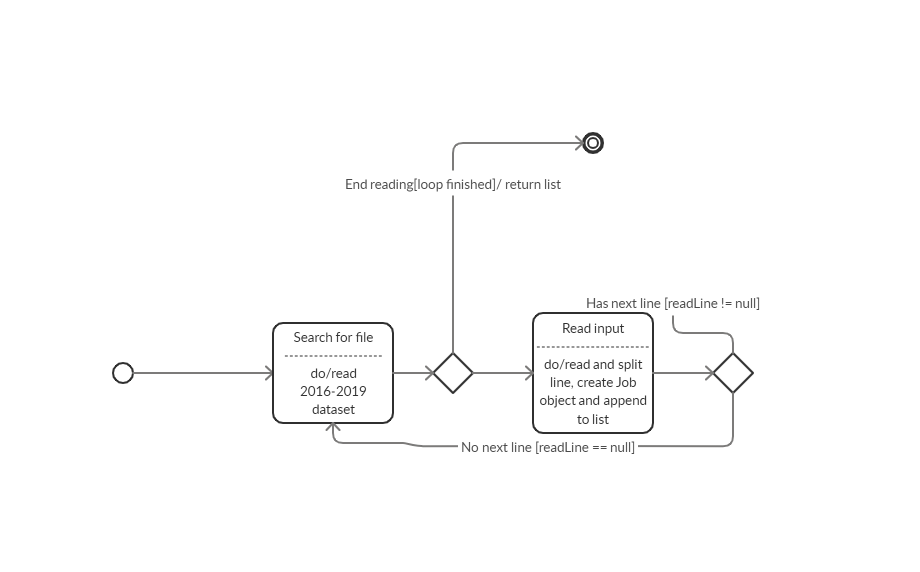
\includegraphics[width=0.8\textwidth]{state machine 1.png}\\
\noindent state machine diagram of DemoClient class
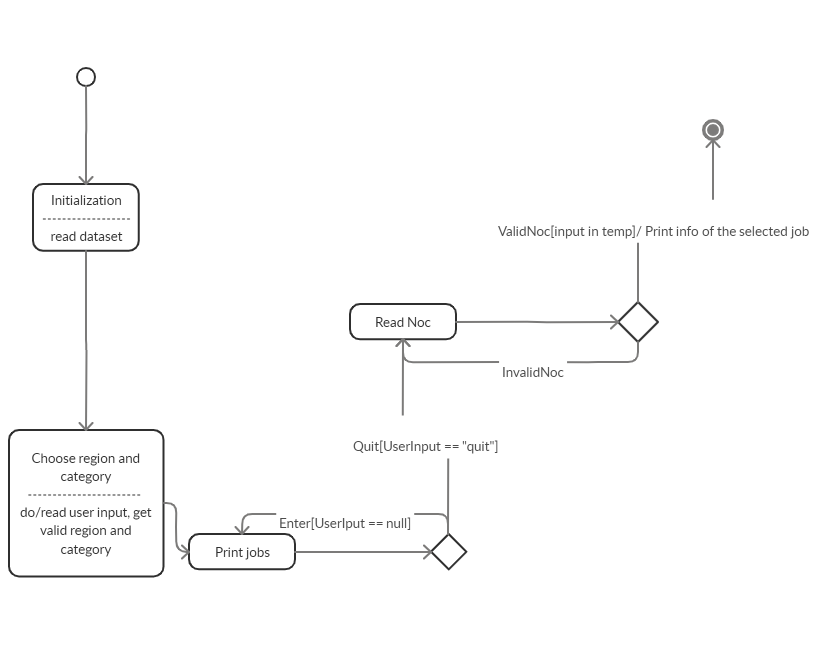
\includegraphics[width=0.8\textwidth]{state machine 2.png}\\
\end{center}
\section{Internal review}
\begin{itemize}
\item JobSeeker is designed to provide information about different kinds of jobs in different regions in recent years for those who are seeking for jobs or investigate the job market. The design is robust and always has a exception class for different illegal inputs. But the user interface is not very user-friendly. It's better to use MVC model here. For the implementaion part, sorting and searching functions are implemented by static functions instead of creating new objects. This reduces the dependency between modules. We put to many methods which we should have separated into different classes in the Demo class like addedge() and read input, which violates the principle of modularity and information hiding. A possible future improvement: allow the user type the region he/she is interested in and find the nearsest region in the dataset using Geocoding API instead of choosing from regions the dataset has.
\end{itemize}

\section{References}
\begin{itemize}
\item GNOME\ Project.\ “An\ Icon\ from\ the\ GNOME-Icon-Theme.”\ WEKIMEDIA\\ COMMONS,\ GNOME,\ 12\ Jan.\ 2008, https://commons.wikimedia.org/wiki/File:Gnome-computer.svg.
\item Sedgewick\ Robert,\ and\ Kevin\ Wayne.\ Algotithms,\ 4th Edition.
\item Open\ Government\ Portal\ (2018, May 15).\ 3-year Employment Outlooks\ .\ Retrieved\ from
https://open.canada.ca/data/en/dataset/b0e112e9-cf53-4e79-8838-23cd98debe5b
\item https://app.creately.com/
\end{itemize}

\end {document}
